\section{Kernel and linear PCA-de-noising on high noise data}
In this section an extreme noise example is considered, where the human eye has trouble identifying the characters correctly.
\begin{figure}
\centering
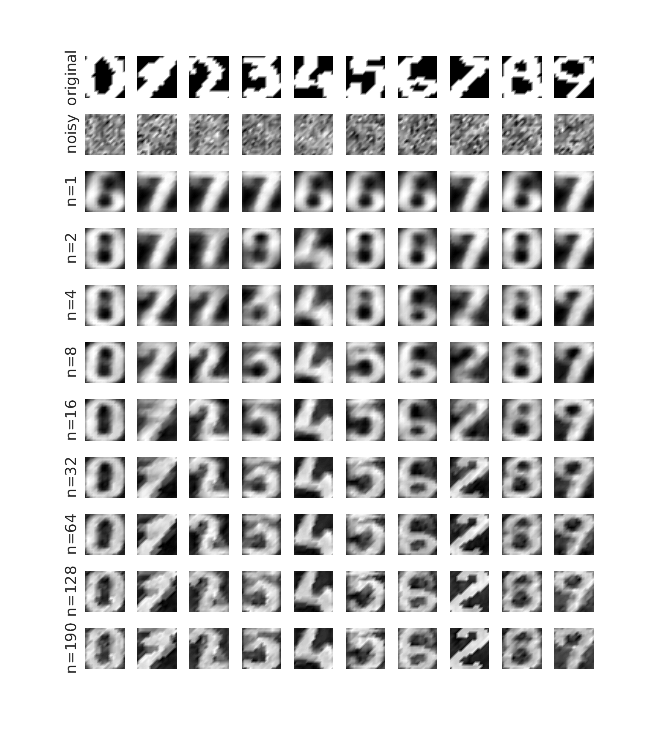
\includegraphics[width=0.45\linewidth]{../src/figure/lotsofNoiseKernel}
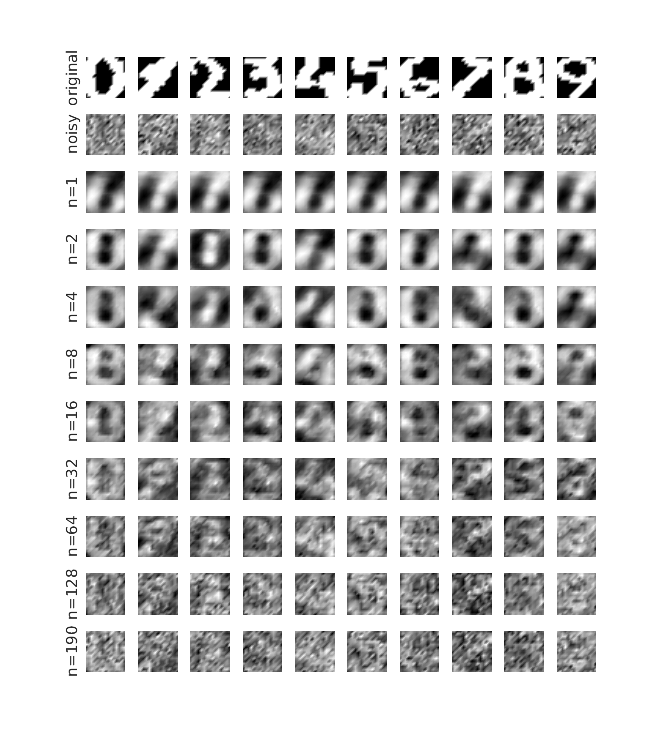
\includegraphics[width=0.45\linewidth]{../src/figure/lotsofNoiseLinear}
\caption{Kernel based and linear pca de-noising of very noise data.}
\label{fig:lotsofNoise}
\end{figure}
Figure~\ref{fig:lotsofNoise} shows the input data as well as the performance of a low sigma kernel-pca in comparison
to a linear one. The trade off that came with choosing the kernel width $\sigma^2$ was observed earlier. A too large $\sigma^2$
led to correct predictions but little noise reduction. Smaller width sometimes ended up clear but incorrect letter representations.
In the case shown in figure~\ref{fig:lotsofNoise} a small $\sigma^2$ had to be chosen in order to deal with the very noisy input.
Given the low quality of the input the kernel-PCA does an incredibly good job at de-noising. It does confuse 3 with 5 and 6 with 2
however. In the linear case this does not happen but it does not come close in terms of noise reduction. 

\section{Shuttle dataset-analysis}
The statlog/shuttle dataset, contains 58000 ten dimensional row data vectors. With the last entry in each row indicating the class to which
the data point belongs. Traditionally the first 43500 data rows are used for training and the last 14500 data points are retained for testing.
\begin{figure}
\centering
% This file was created by matlab2tikz.
% Minimal pgfplots version: 1.3
%
%The latest updates can be retrieved from
%  http://www.mathworks.com/matlabcentral/fileexchange/22022-matlab2tikz
%where you can also make suggestions and rate matlab2tikz.
%
\documentclass[tikz]{standalone}
\usepackage{pgfplots}
\usepackage{grffile}
\pgfplotsset{compat=newest}
\usetikzlibrary{plotmarks}
\usepackage{amsmath}

\begin{document}
\definecolor{mycolor1}{rgb}{0.20810,0.16630,0.52920}%
%
\begin{tikzpicture}

\begin{axis}[%
width=1.5in,
height=1.5in,
scale only axis,
xmin=1,
xmax=7,
ymin=0,
ymax=35000
]

\addplot[area legend,solid,fill=mycolor1,draw=white!15!black,forget plot]
table[row sep=crcr] {%
x	y\\
1	0\\
1	34108\\
1.6	34108\\
1.6	0\\
}--cycle;


\addplot[area legend,solid,fill=mycolor1,draw=white!15!black,forget plot]
table[row sep=crcr] {%
x	y\\
1.6	0\\
1.6	37\\
2.2	37\\
2.2	0\\
}--cycle;


\addplot[area legend,solid,fill=mycolor1,draw=white!15!black,forget plot]
table[row sep=crcr] {%
x	y\\
2.2	0\\
2.2	0\\
2.8	0\\
2.8	0\\
}--cycle;


\addplot[area legend,solid,fill=mycolor1,draw=white!15!black,forget plot]
table[row sep=crcr] {%
x	y\\
2.8	0\\
2.8	132\\
3.4	132\\
3.4	0\\
}--cycle;


\addplot[area legend,solid,fill=mycolor1,draw=white!15!black,forget plot]
table[row sep=crcr] {%
x	y\\
3.4	0\\
3.4	6748\\
4	6748\\
4	0\\
}--cycle;


\addplot[area legend,solid,fill=mycolor1,draw=white!15!black,forget plot]
table[row sep=crcr] {%
x	y\\
4	0\\
4	0\\
4.6	0\\
4.6	0\\
}--cycle;


\addplot[area legend,solid,fill=mycolor1,draw=white!15!black,forget plot]
table[row sep=crcr] {%
x	y\\
4.6	0\\
4.6	2458\\
5.2	2458\\
5.2	0\\
}--cycle;


\addplot[area legend,solid,fill=mycolor1,draw=white!15!black,forget plot]
table[row sep=crcr] {%
x	y\\
5.2	0\\
5.2	0\\
5.8	0\\
5.8	0\\
}--cycle;


\addplot[area legend,solid,fill=mycolor1,draw=white!15!black,forget plot]
table[row sep=crcr] {%
x	y\\
5.8	0\\
5.8	6\\
6.4	6\\
6.4	0\\
}--cycle;


\addplot[area legend,solid,fill=mycolor1,draw=white!15!black,forget plot]
table[row sep=crcr] {%
x	y\\
6.4	0\\
6.4	11\\
7	11\\
7	0\\
}--cycle;

\end{axis}
\end{tikzpicture}%
\end{document}
\caption{Histogram of the statlog dataset's training data class distribution.}
\label{fig:histShuttle}
\end{figure}
Figure~\ref{fig:histShuttle} shows the shuttle-dataset's class distribution. About eighty percent of the data belongs to the first class. 
\begin{figure}
\centering
% This file was created by matlab2tikz.
% Minimal pgfplots version: 1.3
%
%The latest updates can be retrieved from
%  http://www.mathworks.com/matlabcentral/fileexchange/22022-matlab2tikz
%where you can also make suggestions and rate matlab2tikz.
%
\documentclass[tikz]{standalone}
\usepackage{pgfplots}
\usepackage{grffile}
\pgfplotsset{compat=newest}
\usetikzlibrary{plotmarks}
\usepackage{amsmath}

\begin{document}
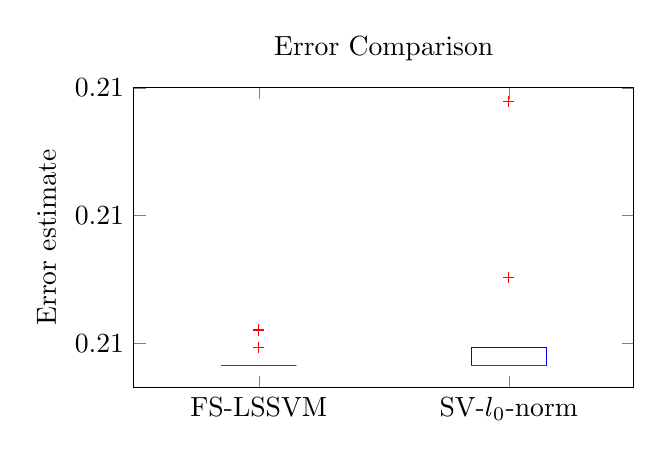
\begin{tikzpicture}

\begin{axis}[%
width=2.5in,
height=1.5in,
scale only axis,
xmin=0.5,
xmax=2.5,
xtick={1,2},
xticklabels={{FS-LSSVM},{SV-$l_0$-norm}},
ymin=0.208326117139843,
ymax=0.209501711991699,
ylabel={Error estimate},
title={Error Comparison}
]
\addplot [color=black,dashed,forget plot]
  table[row sep=crcr]{%
1	0.208413793103448\\
1	0.208413793103448\\
};
\addplot [color=black,dashed,forget plot]
  table[row sep=crcr]{%
2	0.20848275862069\\
2	0.20848275862069\\
};
\addplot [color=black,dashed,forget plot]
  table[row sep=crcr]{%
1	0.208413793103448\\
1	0.208413793103448\\
};
\addplot [color=black,dashed,forget plot]
  table[row sep=crcr]{%
2	0.208413793103448\\
2	0.208413793103448\\
};
\addplot [color=black,solid,forget plot]
  table[row sep=crcr]{%
0.925	0.208413793103448\\
1.075	0.208413793103448\\
};
\addplot [color=black,solid,forget plot]
  table[row sep=crcr]{%
1.925	0.20848275862069\\
2.075	0.20848275862069\\
};
\addplot [color=black,solid,forget plot]
  table[row sep=crcr]{%
0.925	0.208413793103448\\
1.075	0.208413793103448\\
};
\addplot [color=black,solid,forget plot]
  table[row sep=crcr]{%
1.925	0.208413793103448\\
2.075	0.208413793103448\\
};
\addplot [color=blue,solid,forget plot]
  table[row sep=crcr]{%
0.85	0.208413793103448\\
0.85	0.208413793103448\\
1.15	0.208413793103448\\
1.15	0.208413793103448\\
0.85	0.208413793103448\\
};
\addplot [color=blue,solid,forget plot]
  table[row sep=crcr]{%
1.85	0.208413793103448\\
1.85	0.20848275862069\\
2.15	0.20848275862069\\
2.15	0.208413793103448\\
1.85	0.208413793103448\\
};
\addplot [color=red,solid,forget plot]
  table[row sep=crcr]{%
0.85	0.208413793103448\\
1.15	0.208413793103448\\
};
\addplot [color=red,solid,forget plot]
  table[row sep=crcr]{%
1.85	0.208413793103448\\
2.15	0.208413793103448\\
};
\addplot [color=black,only marks,mark=+,mark options={solid,draw=red},forget plot]
  table[row sep=crcr]{%
1	0.20848275862069\\
1	0.208551724137931\\
};
\addplot [color=black,only marks,mark=+,mark options={solid,draw=red},forget plot]
  table[row sep=crcr]{%
2	0.208758620689655\\
2	0.209448275862069\\
};
\end{axis}
\end{tikzpicture}%
\end{document}
% This file was created by matlab2tikz.
% Minimal pgfplots version: 1.3
%
%The latest updates can be retrieved from
%  http://www.mathworks.com/matlabcentral/fileexchange/22022-matlab2tikz
%where you can also make suggestions and rate matlab2tikz.
%
\documentclass[tikz]{standalone}
\usepackage{pgfplots}
\usepackage{grffile}
\pgfplotsset{compat=newest}
\usetikzlibrary{plotmarks}
\usepackage{amsmath}

\begin{document}
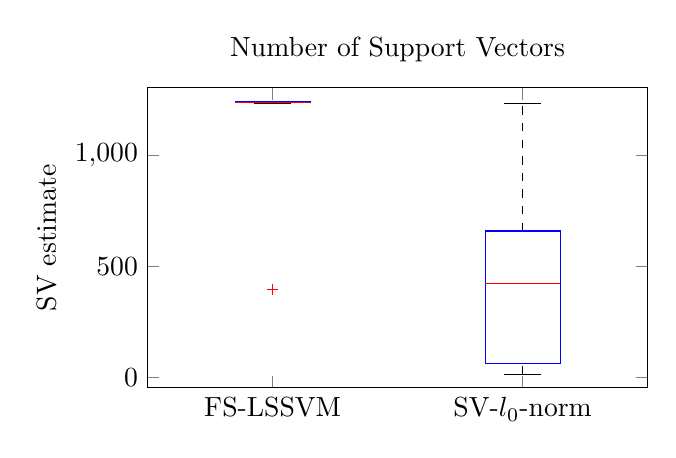
\begin{tikzpicture}

\begin{axis}[%
width=2.5in,
height=1.5in,
scale only axis,
unbounded coords=jump,
xmin=0.5,
xmax=2.5,
xtick={1,2},
xticklabels={{FS-LSSVM},{SV-$l_0$-norm}},
ymin=-46.4,
ymax=1304.4,
ylabel={SV estimate},
title={Number of Support Vectors}
]
\addplot [color=black,dashed,forget plot]
  table[row sep=crcr]{%
1	1241\\
1	1243\\
};
\addplot [color=black,dashed,forget plot]
  table[row sep=crcr]{%
2	660\\
2	1235\\
};
\addplot [color=black,dashed,forget plot]
  table[row sep=crcr]{%
1	1236\\
1	1237\\
};
\addplot [color=black,dashed,forget plot]
  table[row sep=crcr]{%
2	15\\
2	63\\
};
\addplot [color=black,solid,forget plot]
  table[row sep=crcr]{%
0.925	1243\\
1.075	1243\\
};
\addplot [color=black,solid,forget plot]
  table[row sep=crcr]{%
1.925	1235\\
2.075	1235\\
};
\addplot [color=black,solid,forget plot]
  table[row sep=crcr]{%
0.925	1236\\
1.075	1236\\
};
\addplot [color=black,solid,forget plot]
  table[row sep=crcr]{%
1.925	15\\
2.075	15\\
};
\addplot [color=blue,solid,forget plot]
  table[row sep=crcr]{%
0.85	1237\\
0.85	1241\\
1.15	1241\\
1.15	1237\\
0.85	1237\\
};
\addplot [color=blue,solid,forget plot]
  table[row sep=crcr]{%
1.85	63\\
1.85	660\\
2.15	660\\
2.15	63\\
1.85	63\\
};
\addplot [color=red,solid,forget plot]
  table[row sep=crcr]{%
0.85	1237\\
1.15	1237\\
};
\addplot [color=red,solid,forget plot]
  table[row sep=crcr]{%
1.85	425.5\\
2.15	425.5\\
};
\addplot [color=black,only marks,mark=+,mark options={solid,draw=red},forget plot]
  table[row sep=crcr]{%
1	396\\
};
\addplot [color=black,only marks,mark=+,mark options={solid,draw=red},forget plot]
  table[row sep=crcr]{%
nan	nan\\
};
\end{axis}
\end{tikzpicture}%
\end{document}
% This file was created by matlab2tikz.
% Minimal pgfplots version: 1.3
%
%The latest updates can be retrieved from
%  http://www.mathworks.com/matlabcentral/fileexchange/22022-matlab2tikz
%where you can also make suggestions and rate matlab2tikz.
%
\documentclass[tikz]{standalone}
\usepackage{pgfplots}
\usepackage{grffile}
\pgfplotsset{compat=newest}
\usetikzlibrary{plotmarks}
\usepackage{amsmath}

\begin{document}
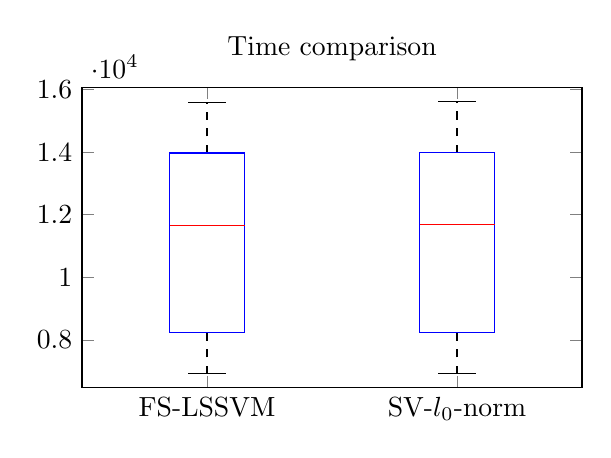
\begin{tikzpicture}

\begin{axis}[%
width=2.5in,
height=1.5in,
scale only axis,
unbounded coords=jump,
xmin=0.5,
xmax=2.5,
xtick={1,2},
xticklabels={{FS-LSSVM},{SV-$l_0$-norm}},
ymin=6472.17200000001,
ymax=16066.988,
title={Time comparison}
]
\addplot [color=black,dashed,forget plot]
  table[row sep=crcr]{%
1	13973.22\\
1	15587.32\\
};
\addplot [color=black,dashed,forget plot]
  table[row sep=crcr]{%
2	13979.24\\
2	15630.86\\
};
\addplot [color=black,dashed,forget plot]
  table[row sep=crcr]{%
1	6908.3\\
1	8218.74\\
};
\addplot [color=black,dashed,forget plot]
  table[row sep=crcr]{%
2	6908.53000000001\\
2	8220.84\\
};
\addplot [color=black,solid,forget plot]
  table[row sep=crcr]{%
0.925	15587.32\\
1.075	15587.32\\
};
\addplot [color=black,solid,forget plot]
  table[row sep=crcr]{%
1.925	15630.86\\
2.075	15630.86\\
};
\addplot [color=black,solid,forget plot]
  table[row sep=crcr]{%
0.925	6908.3\\
1.075	6908.3\\
};
\addplot [color=black,solid,forget plot]
  table[row sep=crcr]{%
1.925	6908.53000000001\\
2.075	6908.53000000001\\
};
\addplot [color=blue,solid,forget plot]
  table[row sep=crcr]{%
0.85	8218.74\\
0.85	13973.22\\
1.15	13973.22\\
1.15	8218.74\\
0.85	8218.74\\
};
\addplot [color=blue,solid,forget plot]
  table[row sep=crcr]{%
1.85	8220.84\\
1.85	13979.24\\
2.15	13979.24\\
2.15	8220.84\\
1.85	8220.84\\
};
\addplot [color=red,solid,forget plot]
  table[row sep=crcr]{%
0.85	11650.65\\
1.15	11650.65\\
};
\addplot [color=red,solid,forget plot]
  table[row sep=crcr]{%
1.85	11674.065\\
2.15	11674.065\\
};
\addplot [color=black,only marks,mark=+,mark options={solid,draw=red},forget plot]
  table[row sep=crcr]{%
nan	nan\\
};
\addplot [color=black,only marks,mark=+,mark options={solid,draw=red},forget plot]
  table[row sep=crcr]{%
nan	nan\\
};
\end{axis}
\end{tikzpicture}%
\end{document}
\caption{Fixed size svm and $l_0$ svm comparison for classification on the nasa shuttle dataset.}
\label{fig:shuttle}
\end{figure}
A modified version of the \texttt{fslssvm\_script} has been used with the shuttle data set as an input. The aim here is again classification, but its must be noted that the shuttle dataset is much larger than the Wisconsin-cancer set, it has 58000 data points while the cancer set only contains 682 data points. The results of the machine architecture comparison are shown in figure~\ref{fig:shuttle}. On this larger data set the difference in terms of the error estimate become negligible. Quite a significance difference in terms of sparsity persist however, while the training time does not increase significantly. 


\section{California dataset-analysis}
The California housing regression problem. Using windowed input data with a delay of 1032, which equals a data size to delay ratio of 20. The same ratio has been successfully applied to the Santa-fe estimation problem. The same experiment is repeated for a regression scenario using the California housing data set. 
\begin{figure}
\centering
% This file was created by matlab2tikz.
% Minimal pgfplots version: 1.3
%
%The latest updates can be retrieved from
%  http://www.mathworks.com/matlabcentral/fileexchange/22022-matlab2tikz
%where you can also make suggestions and rate matlab2tikz.
%
\documentclass[tikz]{standalone}
\usepackage{pgfplots}
\usepackage{grffile}
\pgfplotsset{compat=newest}
\usetikzlibrary{plotmarks}
\usepackage{amsmath}

\begin{document}
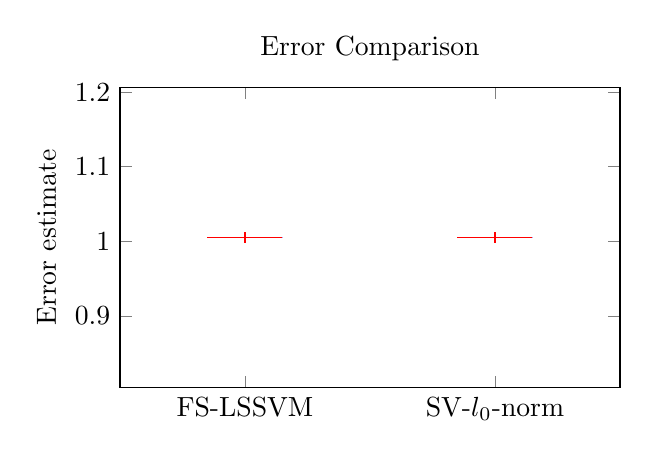
\begin{tikzpicture}

\begin{axis}[%
width=2.5in,
height=1.5in,
scale only axis,
xmin=0.5,
xmax=2.5,
xtick={1,2},
ymin=1.00508302956134,
ymax=1.00508306597566,
ylabel={Error estimate},
xticklabels={{FS-LSSVM},{SV-$l_0$-norm}},
title={Error Comparison}
]
\addplot [color=black,dashed,forget plot]
  table[row sep=crcr]{%
1	1.00508306429705\\
1	1.00508306432046\\
};
\addplot [color=black,dashed,forget plot]
  table[row sep=crcr]{%
2	1.00508306429705\\
2	1.00508306432046\\
};
\addplot [color=black,dashed,forget plot]
  table[row sep=crcr]{%
1	1.00508306415687\\
1	1.00508306415708\\
};
\addplot [color=black,dashed,forget plot]
  table[row sep=crcr]{%
2	1.00508306415687\\
2	1.00508306415708\\
};
\addplot [color=black,solid,forget plot]
  table[row sep=crcr]{%
0.925	1.00508306432046\\
1.075	1.00508306432046\\
};
\addplot [color=black,solid,forget plot]
  table[row sep=crcr]{%
1.925	1.00508306432046\\
2.075	1.00508306432046\\
};
\addplot [color=black,solid,forget plot]
  table[row sep=crcr]{%
0.925	1.00508306415687\\
1.075	1.00508306415687\\
};
\addplot [color=black,solid,forget plot]
  table[row sep=crcr]{%
1.925	1.00508306415687\\
2.075	1.00508306415687\\
};
\addplot [color=blue,solid,forget plot]
  table[row sep=crcr]{%
0.85	1.00508306415708\\
0.85	1.00508306429705\\
1.15	1.00508306429705\\
1.15	1.00508306415708\\
0.85	1.00508306415708\\
};
\addplot [color=blue,solid,forget plot]
  table[row sep=crcr]{%
1.85	1.00508306415708\\
1.85	1.00508306429705\\
2.15	1.00508306429705\\
2.15	1.00508306415708\\
1.85	1.00508306415708\\
};
\addplot [color=red,solid,forget plot]
  table[row sep=crcr]{%
0.85	1.00508306415971\\
1.15	1.00508306415971\\
};
\addplot [color=red,solid,forget plot]
  table[row sep=crcr]{%
1.85	1.00508306415973\\
2.15	1.00508306415973\\
};
\addplot [color=black,only marks,mark=+,mark options={solid,draw=red},forget plot]
  table[row sep=crcr]{%
1	1.00508303121654\\
};
\addplot [color=black,only marks,mark=+,mark options={solid,draw=red},forget plot]
  table[row sep=crcr]{%
2	1.00508303121654\\
};
\end{axis}
\end{tikzpicture}%
\end{document}
% This file was created by matlab2tikz.
% Minimal pgfplots version: 1.3
%
%The latest updates can be retrieved from
%  http://www.mathworks.com/matlabcentral/fileexchange/22022-matlab2tikz
%where you can also make suggestions and rate matlab2tikz.
%
\documentclass[tikz]{standalone}
\usepackage{pgfplots}
\usepackage{grffile}
\pgfplotsset{compat=newest}
\usetikzlibrary{plotmarks}
\usepackage{amsmath}

\begin{document}
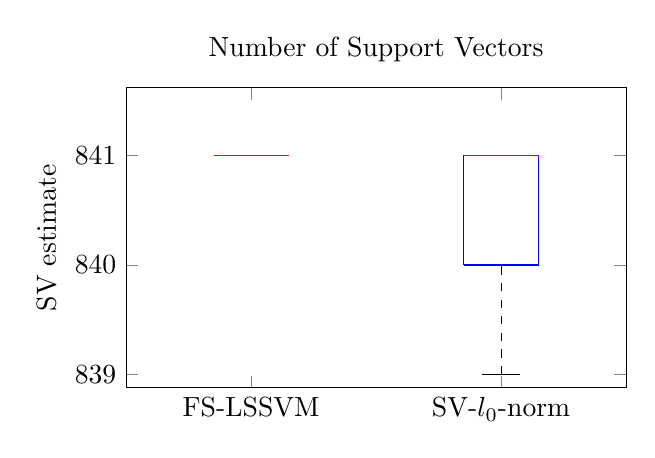
\begin{tikzpicture}

\begin{axis}[%
width=2.5in,
height=1.5in,
scale only axis,
unbounded coords=jump,
xmin=0.5,
xmax=2.5,
xtick={1,2},
ymin=838.875176120368,
ymax=841.621301472279,
ylabel={SV estimate},
xticklabels={{FS-LSSVM},{SV-$l_0$-norm}},
title={Number of Support Vectors}
]
\addplot [color=black,dashed,forget plot]
  table[row sep=crcr]{%
1	841\\
1	841\\
};
\addplot [color=black,dashed,forget plot]
  table[row sep=crcr]{%
2	841\\
2	841\\
};
\addplot [color=black,dashed,forget plot]
  table[row sep=crcr]{%
1	841\\
1	841\\
};
\addplot [color=black,dashed,forget plot]
  table[row sep=crcr]{%
2	839\\
2	840\\
};
\addplot [color=black,solid,forget plot]
  table[row sep=crcr]{%
0.925	841\\
1.075	841\\
};
\addplot [color=black,solid,forget plot]
  table[row sep=crcr]{%
1.925	841\\
2.075	841\\
};
\addplot [color=black,solid,forget plot]
  table[row sep=crcr]{%
0.925	841\\
1.075	841\\
};
\addplot [color=black,solid,forget plot]
  table[row sep=crcr]{%
1.925	839\\
2.075	839\\
};
\addplot [color=blue,solid,forget plot]
  table[row sep=crcr]{%
0.85	841\\
0.85	841\\
1.15	841\\
1.15	841\\
0.85	841\\
};
\addplot [color=blue,solid,forget plot]
  table[row sep=crcr]{%
1.85	840\\
1.85	841\\
2.15	841\\
2.15	840\\
1.85	840\\
};
\addplot [color=red,solid,forget plot]
  table[row sep=crcr]{%
0.85	841\\
1.15	841\\
};
\addplot [color=red,solid,forget plot]
  table[row sep=crcr]{%
1.85	841\\
2.15	841\\
};
\addplot [color=black,only marks,mark=+,mark options={solid,draw=red},forget plot]
  table[row sep=crcr]{%
nan	nan\\
};
\addplot [color=black,only marks,mark=+,mark options={solid,draw=red},forget plot]
  table[row sep=crcr]{%
nan	nan\\
};
\end{axis}
\end{tikzpicture}%
\end{document}
% This file was created by matlab2tikz.
% Minimal pgfplots version: 1.3
%
%The latest updates can be retrieved from
%  http://www.mathworks.com/matlabcentral/fileexchange/22022-matlab2tikz
%where you can also make suggestions and rate matlab2tikz.
%
\documentclass[tikz]{standalone}
\usepackage{pgfplots}
\usepackage{grffile}
\pgfplotsset{compat=newest}
\usetikzlibrary{plotmarks}
\usepackage{amsmath}

\begin{document}
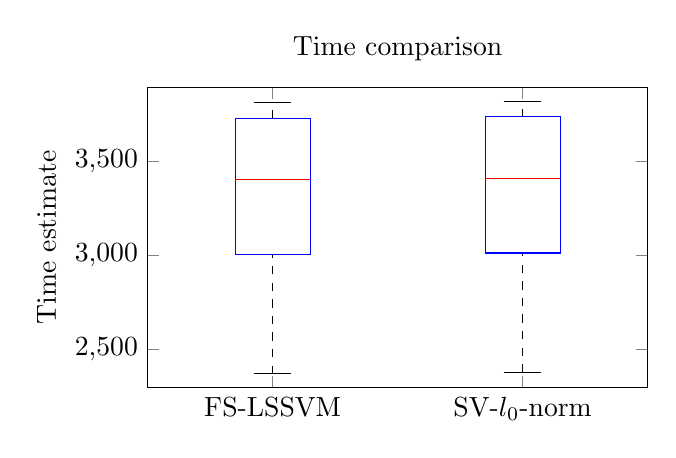
\begin{tikzpicture}

\begin{axis}[%
width=2.5in,
height=1.5in,
scale only axis,
unbounded coords=jump,
xmin=0.5,
xmax=2.5,
xtick={1,2},
ymin=2299.3185,
ymax=3892.1515,
ylabel={Time estimate},
xticklabels={{FS-LSSVM},{SV-$l_0$-norm}},
title={Time comparison}
]
\addplot [color=black,dashed,forget plot]
  table[row sep=crcr]{%
1	3729.47\\
1	3812.98\\
};
\addplot [color=black,dashed,forget plot]
  table[row sep=crcr]{%
2	3736.47\\
2	3819.75\\
};
\addplot [color=black,dashed,forget plot]
  table[row sep=crcr]{%
1	2371.72\\
1	3006.7\\
};
\addplot [color=black,dashed,forget plot]
  table[row sep=crcr]{%
2	2378.72\\
2	3013.73\\
};
\addplot [color=black,solid,forget plot]
  table[row sep=crcr]{%
0.925	3812.98\\
1.075	3812.98\\
};
\addplot [color=black,solid,forget plot]
  table[row sep=crcr]{%
1.925	3819.75\\
2.075	3819.75\\
};
\addplot [color=black,solid,forget plot]
  table[row sep=crcr]{%
0.925	2371.72\\
1.075	2371.72\\
};
\addplot [color=black,solid,forget plot]
  table[row sep=crcr]{%
1.925	2378.72\\
2.075	2378.72\\
};
\addplot [color=blue,solid,forget plot]
  table[row sep=crcr]{%
0.85	3006.7\\
0.85	3729.47\\
1.15	3729.47\\
1.15	3006.7\\
0.85	3006.7\\
};
\addplot [color=blue,solid,forget plot]
  table[row sep=crcr]{%
1.85	3013.73\\
1.85	3736.47\\
2.15	3736.47\\
2.15	3013.73\\
1.85	3013.73\\
};
\addplot [color=red,solid,forget plot]
  table[row sep=crcr]{%
0.85	3402.43\\
1.15	3402.43\\
};
\addplot [color=red,solid,forget plot]
  table[row sep=crcr]{%
1.85	3409.305\\
2.15	3409.305\\
};
\addplot [color=black,only marks,mark=+,mark options={solid,draw=red},forget plot]
  table[row sep=crcr]{%
nan	nan\\
};
\addplot [color=black,only marks,mark=+,mark options={solid,draw=red},forget plot]
  table[row sep=crcr]{%
nan	nan\\
};
\end{axis}
\end{tikzpicture}%
\end{document}
\caption{Fixed size svm and $l_0$ svm comparison for regression on the california-housing dataset.}
\label{fig:california}
\end{figure}
Figure~\ref{fig:california} shows the findings. In this case the a more sparse solution can only be found in some cases. Success in finding a sparse representation probably depends on luck with the random subset the entropy selection method works with.
